\chapter{Measurement of the inclusive $t\bar{t}+\gamma$ cross-section}\label{chap-crosssection}

\section{Signal Definition and Background Processes}

\subsection{Signal definition}

\subsection{Background processes}

\begin{figure}\label{fig-AnalysisFlowChart}
\begin{center}
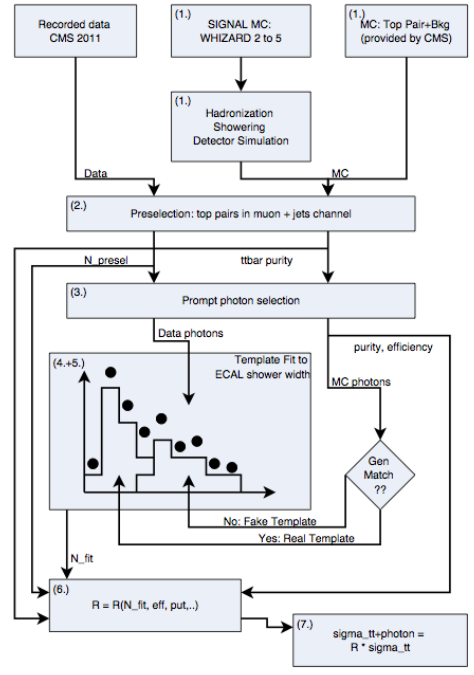
\includegraphics[width=0.75\textwidth]{Figures/AnalysisFlowChart.png}
\caption{Flow chart showing each stage of the analysis. The box numbers represent the outlined
analysis steps.}
\end{center}
\end{figure}

\section{$t\bar{t}+\gamma$ Signal Simulation}

WHIZARD

then

MADGRAPH

Factorised matrix element 

\begin{figure}\label{fig-MatrixElementCalculation}
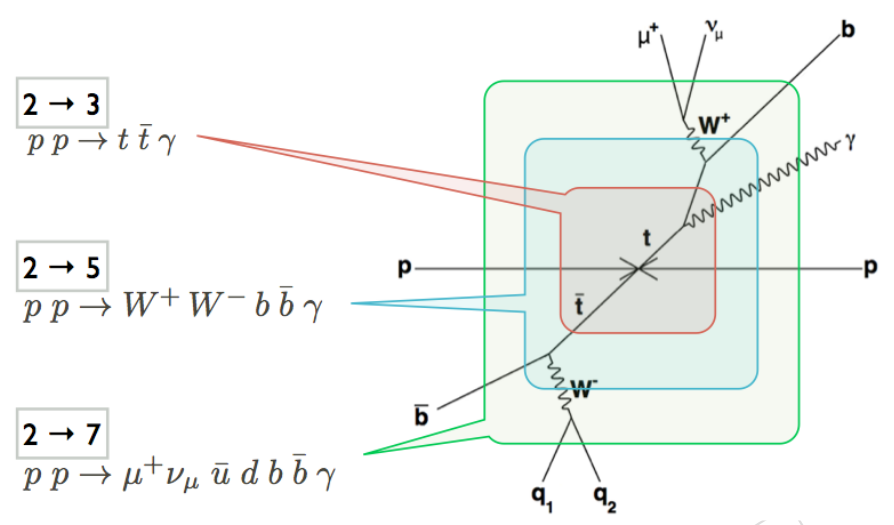
\includegraphics[width=\textwidth]{Figures/MatrixElementCalculation.png}
\caption{Three different methods to define the signal process \cite{heinerthesis}.}
\end{figure}

\section{Phase Space Overlap Removal}

\section{Event Selection}